% !TeX root = ../../main.tex
\documentclass[../AAE590LGM_HW4.tex]{subfiles}
\begin{document}

\begin{figure}[H]
    \caption{Rumoca}
    \centering
    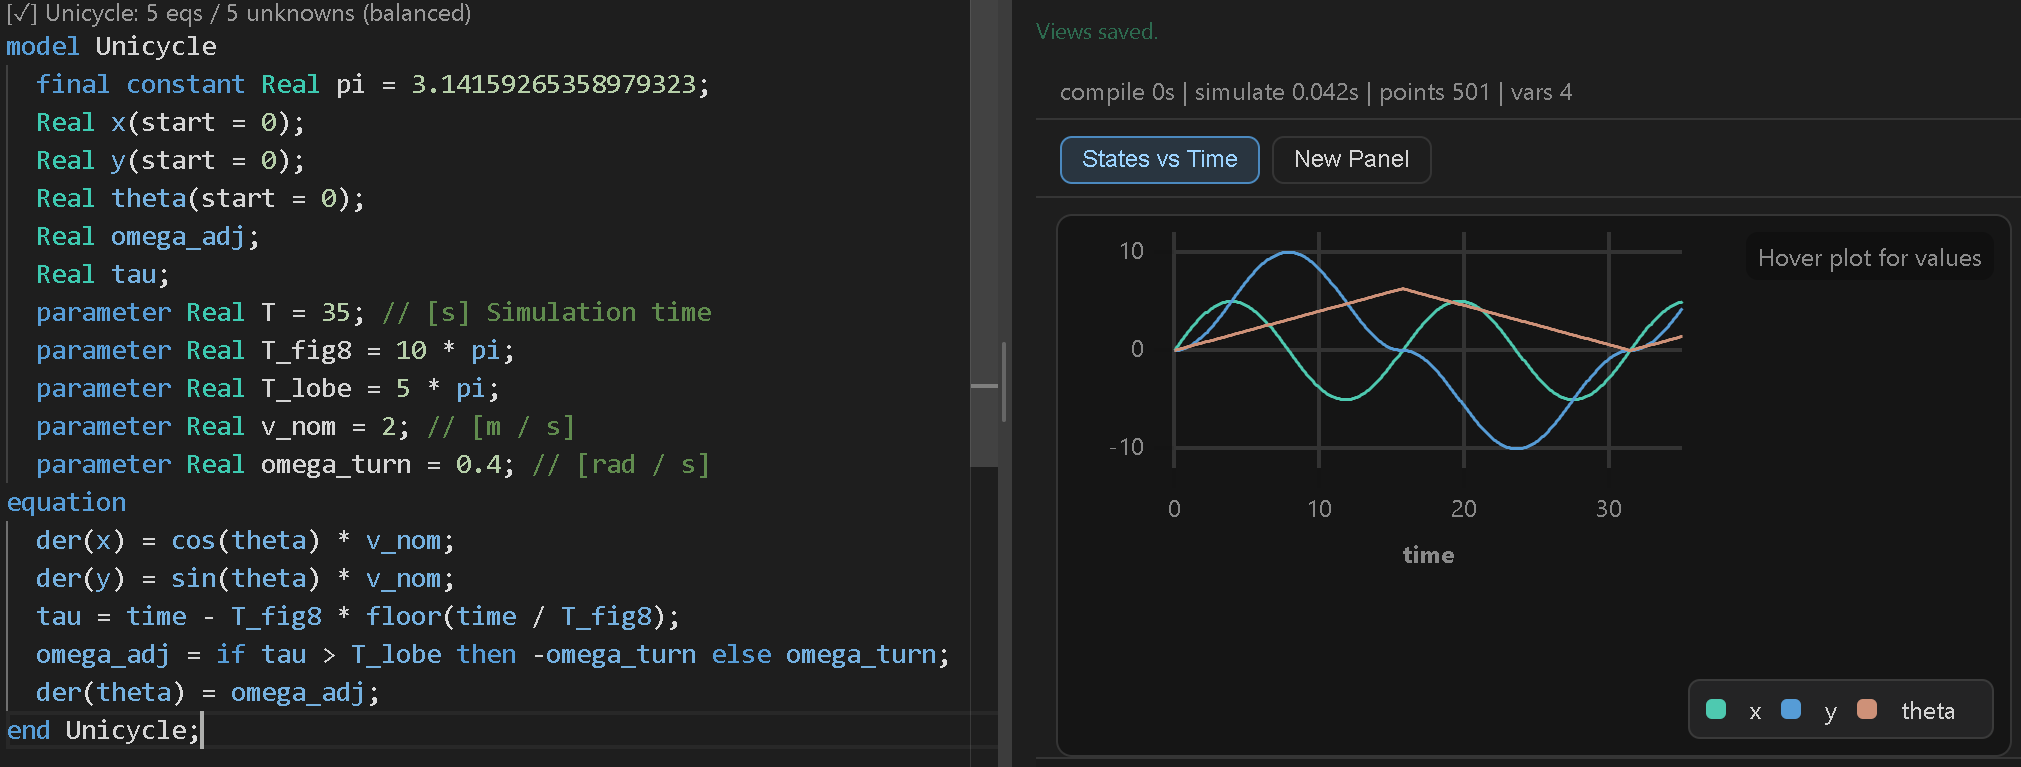
\includegraphics[width=0.7\linewidth]{rumoca.png}
\end{figure}

I did not have time to figure out how to hook up the generated code with a IVP solver. 
It seems like the SUNDIALS4py IVA solver would be ideal since Rumoca uses sundials to solve DAE equations.
The trajectory here is more accurate than what I was using earlier because for my python code 
I was only sampling the twist every 0.1 seconds so it did not flip the angular velocity direction
exactly at the right time, leading to an offset lower lobe. The Modelica trajectory is better 
because it solves the underlying differential equation instead of discretizing it.

\lstinputlisting[language=Python,caption={Rumoca CodeGen}]{AAE590LGM_HW4_Q5.py}


\end{document}